\documentclass[11pt]{article}
\usepackage[top=1.00in, bottom=1.0in, left=1in, right=1in]{geometry}
\renewcommand{\baselinestretch}{1.1}
\usepackage{graphicx}
\usepackage{natbib}
\usepackage{amsmath}
\usepackage{gensymb}
\usepackage{parskip}


\def\labelitemi{--}
\parindent=0pt

\begin{document}
\renewcommand{\refname}{\CHead{}}


\title{The problem and promise of \\ modeling plant leafout under warmer winters} % Infinite models of leafout given warming winters...?
\author{E.M. Wolkovich$^1$, Justin Ngo$^1$, Jonathan Auerbach; plus others possible} % also possibly: Victor van der Meersch, Ron Guy ... Frederik Baumgarten$^1$ though he has been so MIA, I am not sure if he is interested and this paper is unlike the one we proposed to work on together. 
\date{\today}
\maketitle

$^1$ Forest \& Conservation Sciences, Faculty of Forestry, University of British Columbia, 2424 Main Mall, Vancouver, BC V6T 1Z4, Canada\\


\begin{abstract}
Recent evidence of a slow-down in the advance of spring with increasing anthropogenic climate change has reinvigorated a debate over how warmer winters affect plant leafout. Plant biologists have long hypothesized that many woody temperate plants need sufficient winter cool temperatures---or `chilling'---to budburst each spring; thus warmer winters could slow this process and slow advancing spring phenology. But models of this process are many and make diverse predictions for leafout, with different models given the same data often predicting everything from advanced to slowed leafout. Such variability highlights how little we understand the critical process of `chilling,' which is generally never observed but often assumed. Here we show how current work, which routinely models `chilling' with highly limited data has likely led to the proliferation of models---and thus forecasts---and suggest a path forward. We argue that integrating new insights and approaches from molecular biology could push the field to build new models that make falsifiable predictions. This approach could in turn greatly reduce the number of competing models of chilling that we have today------advancing our fundamental understanding of plant dormancy---and lead to better forecasts of leafout and, in turn, climate change. 
\end{abstract}
% ... Such extreme variability of spring phenology predicted from current models suggests fundamental and major gaps in our understanding. Indeed, new research suggests major flaws in these models as currently applied, including multiple papers now suggesting estimates of `chilling' could easily be artifacts of poor models or correlated observational climate data \citep{decsens,gao2024}. 


Plant leafout in the spring has shifted weeks earlier in many regions due to warming from anthropogenic climate change with consequences for a suite of ecosystem services, including carbon storage \citep{keenan2014net,ipcc2022}.  What underlying processes drive this trend, however, has come under increasing debate, as recent research suggests winter warming may slow or stall this advance \citep{fu2015,piao2017}. Such reports focus on a two-step model of leafout where plants first require cool winter temperatures, often called `chilling,' before they can accumulate enough warm temperatures---`forcing'---to leafout each year. But this model of leafout---especially its chilling component---is only one of many models proposed since the concept was first introduced \citep[at least 30 models are used today, see][]{basler2016evaluating,hufkens2018integrated}. 

Current models of chilling predict a full suite of possible future leafout. Chilling in the same location under different models can easily forecast significantly increased or greatly reduced chilling and thus greatly advanced or slowed leafout \citep{guy2014,chuine2016}. Such extreme variability of spring phenology predicted from current models suggests fundamental and major gaps in our understanding. Indeed, new research suggests major flaws in these models as currently applied, including multiple papers now suggesting estimates of `chilling' could easily be artifacts of poor models or correlated observational climate data \citep{decsens,gao2024}. 

Now may be an opportune time to address the problems in models of leafout. Because accurate forecasts of spring phenology are critical for carbon storage, many crops and a number of other services important to humans, there is high interest in improving chilling models \citep{Luedeling2015Acta,chuine2016}. At the same time, new results from molecular and cellular studies of dormancy are providing new insights into when and how chilling works \citep{pan2023epigenetic,zhu2021cold}, which could rule in---or out---some of the myriad current models. 

%FIXME: I need to be more specific! But perhaps do this after a new draft of the paper is done. 
Here, we review the concept of chilling, its origins and potential problems, as well as new opportunities for major advances. In particular, we discuss how new insights from molecular and cellular studies combined with modern approaches to building biological models could revolutionize our understanding of chilling. 

\section*{What is chilling?}

%addbook
How plants in temperature-limited systems avoid leafout during warm spells in the winter has long been debated by plant biologists \citep[e.g.,][]{lamb1948effect,weinberger}. Most work to date has focused on the idea that plants enter some form of dormancy in the fall, which is then released before spring warm temperatures begin. This idea hypothesizes that the slow accumulation of cool temperatures---or chilling---over the winter extends through periods of short warm spells in the winter and thus prevents leafout before spring. 

Much of our fundamental understanding of chilling comes from studies on temperate woody fruit crops where chilling can be critical to yield. Peach trees planted into warmer climates well outside their range (e.g., in Florida or Israel) often have extremely low fruitset because most flower buds do not burst \citep{weinberger,overcash1955effects,erez1971improved}. Initial studies of this phenomenon with related experiments---where cut ends of dormant branches exposed to cooler temperatures in chambers burst more fully and more quickly---underlies most of the models of chilling used today for crops and wild tree species \citep[][]{weinberger,ospreebbms}. %, but these have rarely---if ever---has been well tested. 

The term `chilling' is now used across numerous fields in plant biology to refer to a process where dormant buds exposed to cool temperatures accelerate a phenological event that later occurs after warm temperatures. Focused on how chilling can accelerate events, researchers have calculated `chilling' required for leafout of forest trees from satellite measures of greenup \citep{kaduk2011predicting}, ground observations \citep{Luedeling2009}, and from similar cutting experiments to those used for peaches \citep[reviewed in][]{ospreebbms}.  % A suite of studies on forest trees have also estimated chilling using cuttings of tree branches during the winter in experiments where `chilling' is manipulated either in controlled environment chambers or through the sequential removal of cuttings CITES. While most of these studies focus on leafout, a similar suite of studies on crops has focused on flower burst. 

Alongside these more macro-scale studies of chilling, molecular approaches have also examined chilling, with a wealth of studies on vernalization in \emph{Arabidopsis thaliana}---cool temperatures required for flowering \citep{kim2009vernalization}. These studies generally use controlled temperatures to vary the hypothesized amount of chilling---similar to cutting studies of forest trees and woody crops---then examine molecular and cellular responses \citep[e.g.,][]{pan2021aba,azeez2021early,cai2024molecular}. % Versions of plants with knock-outs of specific genes have helped identify genes that underlie dormancy and other processes related to chilling \citep{songstad2017genome}. 

Today these studies have led to over 30 basic models where accumulated chilling releases plants from dormancy and hundreds or more models considering variation on these models for different species and cultivars \citep[][]{basler2016evaluating,hufkens2018integrated}. Though early debates considered whether plants were truly dormant or only growing slow \citep[`dormancy' or `rest' versus `quiescent;][]{considine2016language}, today most research assumes a model with two phases of dormancy (Fig. \ref{fig:modelsketch}). 

In most models, chilling can only be accumulated under certain temperatures---often above zero but below 10\degree C---with certain temperatures being optimal for the most rapid accumulation of `chill units,' where some unknown sum of chill units breaks endo-dormancy. This mirrors growing degree days in many ways, where a lower temperature (e.g., 5 or 10\degree C base temperature) is too cold for forcing units to accumulate and plants need some total sum of such units to leafout or flower, but has added complexity given the importance of both a lower and upper temperature threshold for `chill units,' and the hypothesized diversity of these temperature thresholds and sums across species and populations. Most assume different species require different sums of chill units, and may have different lower, upper and optimal chill temperatures. Within species, populations may require different sums of chill units, with populations in more mild climates---where warm interruptions in the winter are more common---requiring more chill units than those in areas with cold winters that rarely warm much above zero before spring \citep{campbell1979,leinonen1996dependence}. 

\section*{The problem with chilling} 

Experiments and models focused on chilling describe an unobserved process \citep{chuine2016,chuinearees}, with critical differences between the two approaches. In most models the term `chilling' describes a process that occurs when plants are in a specific physiological phase and experiencing environmental temperatures known to induce progress towards the next physiological state. In an experimental context, however, the term `chilling' often refers to a treatment where researchers do not know the physiological phase of the plant \citep{flynn2018,ospreebbms}. For example, cuttings or buds are often chilled at 5\degree C for 6 weeks in the dark in a `chilling' treatment, then transferred to warming `forcing' conditions without information on physiological phases. While this may seem like a small terminology issue it actually belies one of the major problems with our understanding---and thus modeling---of chilling today, which is the complexity of measuring an unobserved process with so many unknowns \citep{ospreebbms}. %FIXME -- ref box with JA model in this paragraph and maybe extract out some of 'cuttings or buds are often chilled...' sentence.

Most current models of chilling try to estimate a large number of unknowns---generally as model parameters---from data that yields limited inference. A simple model would need to estimate the minimum and maximum temperatures that allow chilling to accumulate (two parameters) and the total sum of those temperature units needed to trigger endo-dormancy break (one additional parameter for three total). Models then need to estimate  when plants start and stop accumulating (two more parameters), but this is generally intractable (see BOX). To address this, models today assign the start date as known (e.g., starting 1 September in the Northern Hemisphere) and rely on assumptions to set the end date. A common assumption, developed by early work on peaches, is that high and rapid leaf or flowerburst is evidence that chilling has been met \citep{erez1971}. While this assumption is widely used, it is rarely if ever tested beyond the early work on peaches. This approach of assigning some unknown parameters as known (without any variance) has the benefit of avoiding adding more unknown model parameters, but it also has led researchers to be overly confident in a model for leafout where more is actually unobserved and unknown than acknowledged. % FIXME -- ref box here and below

Hidden assumptions and numerous parameters can easily drive diverging models. Even if we assume percent leafout or flowerburst signals sufficient chilling most models today include parameters that cannot be uniquely identified with current data (see BOX).  Given experiments and models have suggested many variants on a more complicated model of chilling---for example minimum, maximum and optimal temperatures, or high temperatures that reduce previous accumulation \citep[Fig. \ref{fig:modelsketch}][]{lued2011,luedeling2012chilling,chuine2016}---current data are relatively uninformative to try to estimate all the parameters the models include. Further, recent models have often relied on even less data; many current methods use only observational data of the timing of leafout (or flowering) to attempt to estimate a model of chilling for different species or locations and project it forward to understand effects of anthropogenic climate change \citep{lued2011,luedeling2012chilling,gao2024}. Perhaps not surprisingly then, which model is deemed best varies strongly by method and approach CITES, with no clear pattern. 

\section*{New molecular insights could reshape the field and its models} 

% Molecular insights have long helped crop and forest tree models of chilling CITES, but recent findings appear especially promising to build a more unified and coherent model. 
Molecular insights have long helped crop and forest tree models of chilling \citep{chuinearees}. Decades of work on vernalization have outlined the pathways---and genes---that lead to flowering only after winter's cool temperatures in biennial (herbaceous) populations of \emph{Arabidopsis thaliana} \citep[Fig. \ref{fig:molecular}][]{Wilczek:2009oa,kim2009vernalization}. Research has linked these some of these pathways to similar ones in woody species, but have also highlighted the sugar callose (1,3-$\beta$-{\sc D}-glucan) as potentially pivotal for chilling. Multiple studies across multiple species have now shown that (1) lower temperatures appear to degrade callose and (2) the release/loss of callose appears to re-start cell-to-cell communication before budburst \citep{vanderschoot2014}. Taken together, these results suggest the loss of callose---generally degraded through 1,3-$\beta$-glucanases (a group of enzymes)---may be an indicator of endo-dormancy release \citep[though other factors (e.g., ABA) also often change at the same time,][]{tylewicz2018photoperiodic,pan2021aba} and may provide a similar observable signal of endo-dormancy release. \citep{rinne2018,andre2022populus}. 


% New cellular and molecular results could potentially reduce this complexity, and help narrow the set of possible models.  We argue that two new major insights from molecular studies---the importance of callose and temperature-dependent growth---could limit the chilling models considered today, and reshape the experiments tree biologists use to determine `chilling.' 

% MOVE this text to a figure caption maybe?
% The hypothesis that the sugar callose may play a pivotal role in bud endodormancy has been suggested for over a decade \citep{rinne2011}, but recent studies have yielded increasing support for this hypothesis \citep{vanderschoot2014,pan2023epigenetic}. Callose (1,3-$\beta$-{\sc D}-glucan), which is synthesized for various reasons in plants (e.g., at the site of infection to prevent pathogens), also appears to block plasmodesmata in dormant buds. 

If callose is functionally a major controller of endo-dormancy and its release it suggests chilling models could be limited to those that match the idea of glucanase degrading callose---meaning models that include a temperature range over which the enzyme is active. In contrast, models using simple temperature thresholds (e.g., all hours below -5\degree C equally allow chilling) would appear less biologically accurate, as enzymes generally do not work over such a wide range of temperatures. Other new molecular insights similarly suggest simplified temperature metrics may not map to molecular realities. For example, new work on how slow growth itself may act  a `long-term thermosensor' \citep{zhao2020temperature} adds to an increasing number of molecular studies that suggest plants integrate long-term thermo-sensing in the winter alongside responses to short-term temperatures \citep{antoniou2021feeling,Satake2022}. The best models of leafout may thus need to integrate across multiple timescales.This could easily add complexity to models of spring phenology that are already challenged by too much complexity. But we argue that new insights from molecular biology could begin to rule out models by focusing on new experiments and modeling approaches that target the major problems facing models of chilling. % especially given how little of the dormancy process we currently observe.  


% Models of chilling and forcing CITEFiG generally assume accumulation processes, mirroring processes that may occur at the cellular level (e.g., accumulation of callose, followed by accumulation glucanases that degrade it). 
% Another major insight from molecular studies suggests that temperature-dependent growth may determine the build-up---or dilution---of cellular components (e.g., proteins) that determine dormancy \citep{zhao2020temperature,antoniou2021feeling}. While many molecular models focus on conditions that increase protein synthesis, new research suggests temperature dependent growth could explain patterns of accumulation and dilution in proteins that trigger vernalization \citep{zhao2020temperature}. In this way, slow growth in the winter may act as a `long-term thermosensor.' If these results hold up across other studies and species, they would suggest that temperature synthesis ranges and optima for different molecules may be less apparent---and potentially less critical to model---when growth regulates concentration \citep{zhao2020temperature}.
% Something about how both callose and temperature dependent growth mean you could go forward and then back (lose callose... gain it back), which adds complexity ... but has been long hypothesized ... but also means models alone without better observed data in experiments will NEVER save us. 




\section*{Building a better model of chilling} % 2700 words, so need to get this wrapped up in < 2K words


Perhaps the most important way to leverage new molecular insights for progress on chilling models is through new experiments that redefine chilling through testing for robust markers of physiological shifts in the winter. Experiments testing for evidence of callose loss using common temperature treatments of past studies (CITEMEospree) currently appear most promising, but could be complemented by looking for other cellular and molecular indicators (citeWENDEN?). Testing these methods together alongside previous-used markers of dormancy shifts---including the often-used bioassay of high and rapid budburst at higher temperatures (indicating endo-dormancy release), and additional methods, such as weighing flower buds \citep{chuine2016} or tracing water reactivation into cells \citep{faust1991bound,Kalcsits2009}---could help align both new and old methods. Because chilling is functionally an unobserved process we argue that comparing methods should be a major priority for the field. This comparison will need to allow for the reality that different methods may measure different processes and we ague that terminology may need to adapt as well. As a first step, research needs to stop referring to treatments in experiments as `chilling' or `forcing' or other terms that assume an underlying physiological state, and instead focus on the actual treatments (e.g., `cool temperatures before warm'). 
%  Testing some of these methods together with cellular and molecular indicators should be a major priority for the field, though researchers will need to evaluate their effectiveness carefully, especially as cellular and molecular insights will likely come from different species than those often modeled and possibly for different events (e.g. for flowering when the many models focus on leafout). % And see BOX on what is wrong with current methods?
% While a number of recent paper papers, have reviewed molecular advances in research related to chilling CITES, sometimes explicitly with an aim to bridge to models of tree chilling (Zhang et al 2023), they often review a diversity of advances. 

% START HERE! 
% I think the two below sentences go with above paragraph ... decide what to do with them. And then dive in on next paragraph (from outline: new generation of experiments [bridge fields, measure more temperatures in molecular -- I started this below!] and what old experiments could do ...) 
Perhaps the most important way to leverage new molecular insights for progress on chilling models is through new experiments, designed to identify markers of the underlying physiological stage ... 
Perhaps the largest problem with current models of chilling is their non-identifiability. 

Progress through new experiments could come from more approaches that bridge across molecular and phenological methods in not only what they measure .... 

% While previous models of chilling have attempted to integrate some of these insights into other tree species \citep{landsberg1974apple,Kramer1994}, they often resulted in adding additional, more complex, models of the chilling to the long list of existing models \citep{hanninen1990modelling}. 

% Moving from first section, and dropping it here for now! 
One way to increase the amount of data used to estimate chilling models would be to include both experimental and observational data together in one model, but this has never been done to our knowledge. Instead, models continue to infer parameters from other data or studies, then fit only certain parameters of their models to a dataset at hand \citep{richardson1974}. While conditions in observational and experimental are often different---for example, many experiments apply cold temperatures in the dark, while photoperiod shifts each day in observational data---continually fitting the resulting data separately slows progress towards a coherent model and contributes to the increasing diversity of proposed models today. 

% Taking this from above and dropping it here for now! 
New molecular insights hold promise to remove part of the non-identifiability. Thus, we argue that experiments attempting to assess chilling should begin testing for callose loss or other  cellular and molecular indicators alongside previous-used markers. This includes the often-used bioassay of high and rapid budburst at higher temperatures indicating endo-dormancy release, and additional methods, such as weighing flower buds \citep{chuine2016} or tracing water reactivation into cells \citep{faust1991bound,Kalcsits2009}. Testing some of these methods together with cellular and molecular indicators should be a major priority for the field, though researchers will need to evaluate their effectiveness carefully, especially as cellular and molecular insights will likely come from different species than those often modeled and possibly for different events (e.g. for flowering when the many models focus on leafout). % And see BOX on what is wrong with current methods?
% While a number of recent paper papers, have reviewed molecular advances in research related to chilling CITES, sometimes explicitly with an aim to bridge to models of tree chilling (Zhang et al 2023), they often review a diversity of advances. 

We argue that better models of chilling are possible given new insights alongside new approaches to how we model---and communicate---models of chilling. Models assumptions and identifiability need to be more clearly explained. This includes clearly defining chilling and endo-dormancy or similar transitions and how they are measured from data used to inform or parameterize models. As most current models of chilling appear non-identified---where all parameters cannot be clearly estimated from given data---more open review and discussion of this could greatly help compare models. 

Clear assumptions and non-identifiability often go together, a relationship that should be clearer in models. For example, making an assumption that chilling can only occur within a narrow range of temperatures may make it possible to estimate both these temperatures and the total sum of required chilling for endo-dormancy release, but relaxing the temperature range assumption would make these two components non-identified. Given the extensive list of proposed complexities to chilling models (see Box), having simpler models (fewer parameters) that are routinely used to compare to more complex models, would likely help the field advance. Currently, very simple models often outcompete more complex models, suggesting how we advance from these simpler models is also a problem \citep[e.g.,][]{basler2016evaluating}. 

Models are often tested on observational phenology data, which may explain why simpler models often appear to perform well. Many studies suggest that `natural' field conditions should satisfy chilling requirements for wild species, thus models without any chilling may perform well. The concept of chilling was developed, however, from experiments and from crop species planted well outside their natural range. Tests of chilling models thus, should include a suite of data types. At a minimum comparisons should include observational data and experimental data---models that cannot fit both data types should be flagged as indicating a problem with the model.  At the same time, datasets must provide the necessary information to fit chilling models (e.g., for experiments---what was the dormancy induction temperature, what as the thermo and photo-periodicity of each stage of the experiment). 
% This makes sense in an evolutionary sense, as species should evolve chilling such that allows endo-dormancy break well in advance of spring conditions, but is difficult to test when we do not know clearly what chilling or endo-dormancy break are physiologically. 

Changing how we evaluate and compare models should make it possible to discard models more often. To date, models are often compared using model comparison statistics and using different datasets in different papers. We argue that these two approaches make it virtually impossible to advance the field, since one model may be preferred on some data for certain model statistics and another model given other data and statistics. Building standard datasets that are always tested alongside expected certain test statistics would alleviate some of this problem, and make it easier to identify why different datasets find different answers. 


Discarding models likely requires moving away from model comparisons statistics and towards designing models that make falsifiable predictions. For example, molecular biologists tested their vernalization model by through comparing predicted to observed flowering times in common garden study across Europe \citep[][]{Wilczek:2009oa}, and supported the temperature-dependent growth model by testing its predictions of what happens when growth is altered but temperature is held constant \citep{zhao2020temperature}. Similar examples for challenging other models of chilling date back over 40 years to when many of the models were developed (addCITES), but could take place now. Models of chilling can make predictions under lower field chilling then test them using individuals planted beyond the range (either planting those individuals now or identifying such cases in forestry provenance trials or similar). 

Building models with falsifiable predictions is standard in molecular biology and highlights how working across these disciplines could especially advance both fields of research into chilling. In addition to leveraging molecular insights to determine what model structures best align with our current understanding of physiological dormancy and its release, more efforts to measure compounds related to dormancy release could reshape how we model it. It may be that the field's long reliance on rapid and high percent budburst under warm temperatures only aligns with physiological dormancy release for some species and/or conditions. Similarly, synthesizing models---and their underlying biological understanding of chilling---across the many field developing chilling models today could eventually reduce the total number of models to compare. Currently, crop biologists, phenological process-based modelers of forest trees, molecular biologists and hardiness modelers all develop unique and rarely compared models of dormancy and budburst, highlighting a big problem, but also a major opportunity. Uniting these models, first by fully defining their assumptions and conditions (e.g., what species are they designed for, what phenological or dormancy phase do they start at?) then comparing their predictions and pushing them to make different testable predictions seems an obvious path to building a unified model of chilling, with implications for much better models of budburst, and cascading improvements in forecasts for crop yield to forest carbon sequestration. 
% Current advances in the molecular biology of chilling hint that some components of current chilling models may wrong---based on our current understanding---but fully debating this would take more interdisciplinary efforts. 

\vspace{10ex}

{\sc Box: Non-identifiable models} % May need a better title

Experiments assign treatments as `chilling' and `forcing' ... the actual physiological transition may occur in the cool `chilling' treatment or much later in the warm `forcing' conditions. ...
These models often assume when to start and stop accumulating, based on much earlier work often done only on crops. Early models of chilling---done mostly on peaches and other woody crops---tried to estimate the physiological phase of chilling by using experimental data of percent leaf or flowerburst as evidence that chilling has been met, then attempted to identify the range of temperatures where chilling accumulates \citep{erez1971}. Taking these estimated temperatures, they then used field observations of percent flowerburst for plants across a wide range of climates---including those well outside the natural range where percent flower burst in many years was low---to estimate the total chilling needed for different cultivars \citep{richardson1974}. This approach of using separate datasets to estimate different parameters of what should be one coherent model laid the groundwork for models today where a number of assumptions or parameters are made directly without be questioned or examined. ...
In this way, separate datasets were used to estimate different parameters of what should be one coherent model, an approach that has persisted today, and one that hints at the non-identifiability of current models given our data and knowledge. 
% Current methods use limited data to estimate a hypothesized accumulation that triggers an unobserved event---currently often described as the release of endo-dormancy---which then leads to another accumulation that leads to leafout or flowering. 



{\sc Box: What we know matters to chilling, and what might matter} % and why we keep going around in circles on negative temperatures?

Studies on how cool winter temperatures affect budburst have identified numerous possible factors that appear to moderate `chilling.' Certainly time and cool temperatures affect budburst timing. Teasing out the effect of time versus temperature has proven difficult, but plants and cuttings (clipped ends of tree branches with one or more bud) exposed for the same amount of time to different constant cool temperatures budburst at different rates and percentages CITES. Which temperatures are most effective at providing chilling---estimated as those that lead to either (or both) the highest percent or fastest budburst after exposure to warm (often 20\degree C) temperatures---is a common question addressed in experiments, with different experiments providing different answers CITES. 

This has led to debate recently on whether sub-zero temperatures can provide chilling as one recent studied appeared to show \citep{baum2021}, supporting previous research \citep{Jones:2012,Sonsteby:2014aa}, but in contrast to other studies \citep{lamb1948effect,cook2005freezing,Man:2010aa}. These studies, however, vary in a number of additional factors including the species they study, the full conditions under which cool temperatures were applied etc.. This debate highlights the complexity of identifying the dominant controllers on chilling when so many factors vary across studies, and so many factors appear to moderate effects. In addition to the temperature range, temperature variability also appears to play a role CITES. The role of sub-zero temperatures and temperature variability also matter strongly to plant hardiness---what level of cold temperatures plants can withstand without damage, which is induced alongside dormancy in the fall for most temperature species. Recent work by \citet{kovaleskipreprint} has reignited an old debate about whether hardiness influences dormancy CITES---or vice versa. 

% Maybe cut the below? Seems annoying nanny-like text (says the person who wrote it)
These debates---about the importance of sub-zero temperatures and plant hardiness to dormancy and chilling---are not new, and also highlight gaps in the approach many biologists have taken to studying chilling in an era where how well we understand it has major implications due to anthropogenic climate change. Some recent papers  ask similar questions to those of decades ago, often failing to cite the earlier literature \citep[e.g.,][]{lamb1948effect,Man:2010aa,baum2021}. While this highlights that such debates may not have been fully settled it can also slow progress. Because of this, we suggest a major need is to build and share databases of all relevant studies---across molecular, crop, and forest biology. Such databases should include information on factors that appear to effect chilling, including dormancy induction temperature, species, provenance location  \citep[as different populations may need different chilling][]{campbell1979,leinonen1996dependence}, thermo- and photo-periodicity of all applied treatments, and any hardiness information. We provide a start to this in the supplement. % Maybe ...  

% While better documenting the diversity of species and treatments applied in chilling-related studies to date will help, progress may require a greater focus on solving the problem for one species ..... 

\vspace{5ex}
{\sc Possible other Box: The problem with how we measure endo-dormancy release currently} % could also include that we don't measure it much

 Traditionally, experiments to test for effective chilling temperature ranges in woody species have used a heuristic where budburst that is rapid and includes a high percentage of buds bursting indicates endo-dormancy release has happened. This method has the benefit of being a useful bioassay---testing if plants can budburst as a metric of an endo-dormancy release (indeed, this method and the term were developed together, CITES)---but has disadvantages in that the method, which works well for some stone fruits, often appears much messier in other species. Because the method relies on fitting a hypothesized curve (or simple threshold) to set a date or level of for endo-dormancy break, how well it performs for many species is often not clear CITES, and thus whether it is an accurate bioassay is similarly unclear. For this reason, others have argued for other methods, such as weighing flower buds \citep{chuine2016}CITES or tracing water reactivation into cells \citep{faust1991bound,Kalcsits2009}. 

% Bad things without a home ...
% And then there are attempts to estimate chilling using observational data in crops (but often when planted outside range) and forest trees ... and basically always based on assumptions from existing models and/or experiments (peaches again).

\clearpage
\bibliographystyle{/Users/Lizzie/Documents/EndnoteRelated/Bibtex/styles/besjournals}
\section{References}
\bibliography{..//refs/bibforchillingconceptms}


\clearpage
\section{Figures}

\begin{figure}[h!]
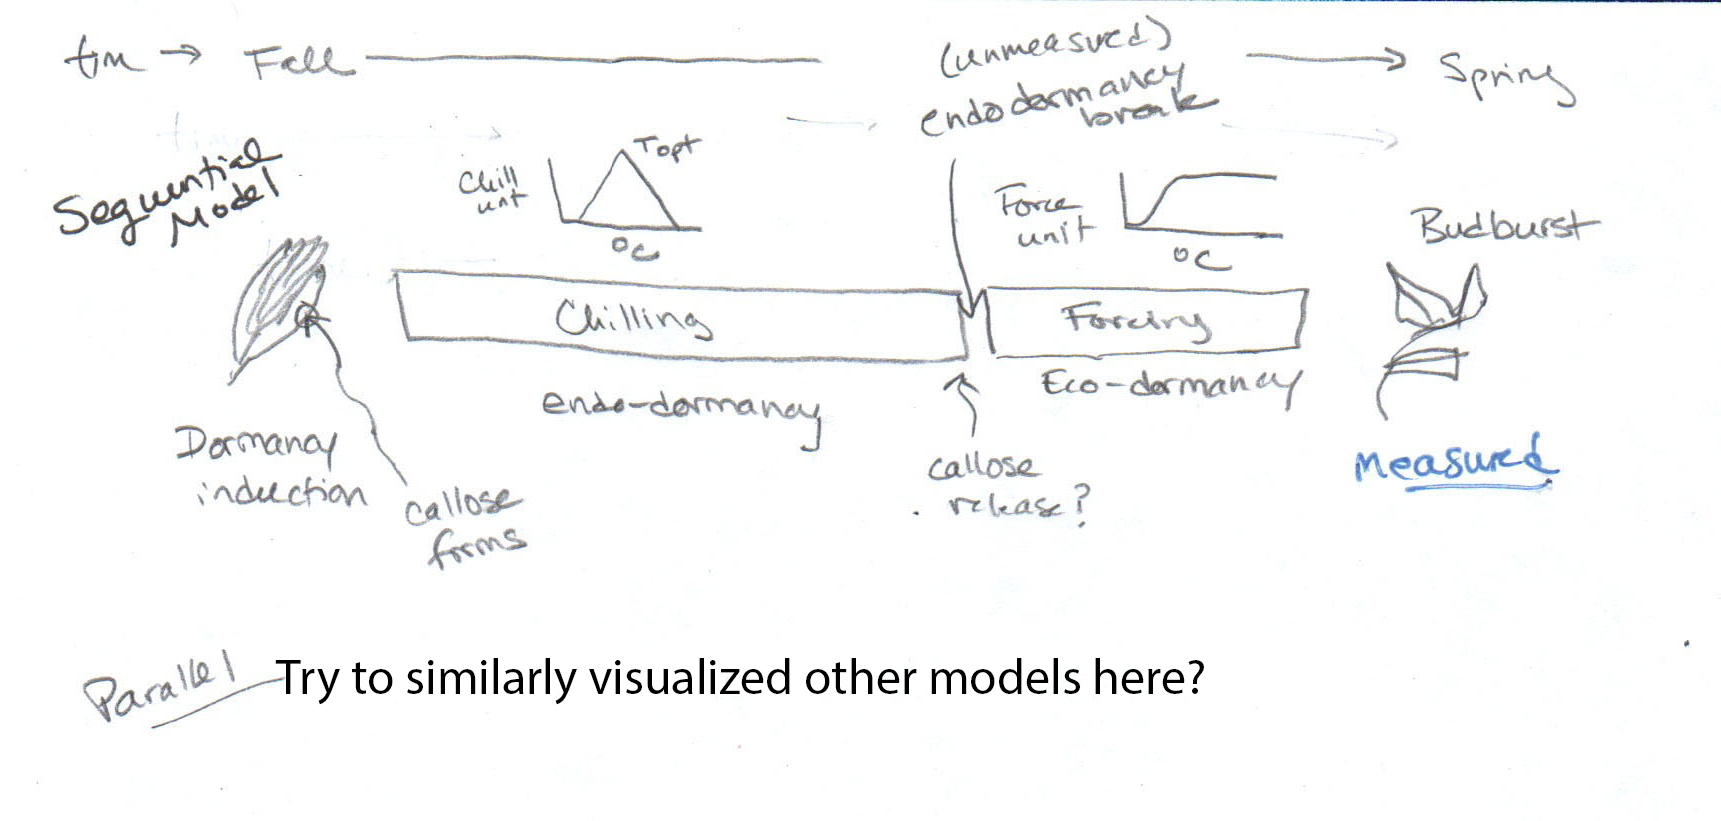
\includegraphics[width=1\textwidth]{..//figures/chillingmodel_drafttext.png}
\caption{Draft idea of how to visualize simple sequential model but layering on physiological stages, some of the model parameters (not fully shown, but could go with small graphics above `chilling' and `forcing'), what is measured, and callose. I wanted to add other models, like the parallel, but was not sure how. I can work on that if we want to keep this figure idea.} 
\label{fig:modelsketch}
\end{figure}

\begin{figure}[h!]
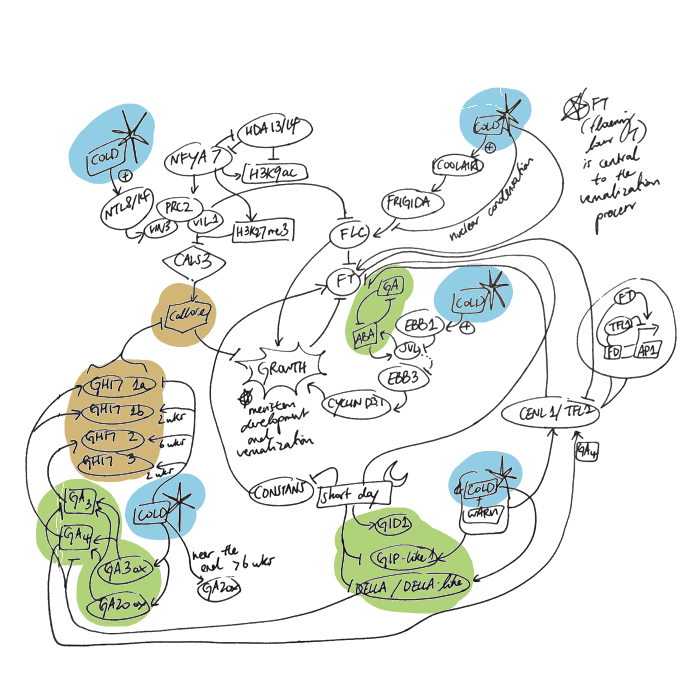
\includegraphics[width=0.9\textwidth]{..//figures/biochemicalModelSketch.png}
\caption{Draft visualization of molecular pathways identified in vernalization and chilling; if we want to keep this, we can update to clarify which have been found in woody species perhaps and match the text a little more. ADD to caption: In the first phase---endo-dormancy---plants are accumulating `chilling' and cannot respond to external warm periods  \citep[thus the `endo' part of the term,][]{chuine2016,lundell2020}. Once they have accumulated the appropriate amount of `chilling' they are `eco-dormant,' and will leaf or flower in response to a sufficient thermal sum (often called forcing, or `growing degree days' in some models). } 
\label{fig:molecular}
\end{figure}

\end{document}
